
\begin{figure}[!htb]
	\centering
	\resizebox{0.5\columnwidth}{!}{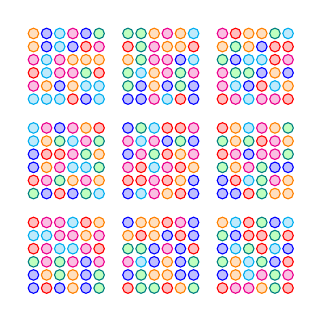
\begin{tikzpicture}
\draw[draw=blue, fill=blue, fill opacity=0.25] (1.3666666666666667, 1.3666666666666667) circle (0.06666666666666667);
\draw[draw=blue, fill=blue, fill opacity=0.25] (1.3666666666666667, 1.5333333333333332) circle (0.06666666666666667);
\draw[draw=teal, fill=green, fill opacity=0.25] (1.3666666666666667, 1.7) circle (0.06666666666666667);
\draw[draw=red, fill=red, fill opacity=0.25] (1.3666666666666667, 1.8666666666666667) circle (0.06666666666666667);
\draw[draw=cyan, fill=cyan, fill opacity=0.25] (1.3666666666666667, 2.033333333333333) circle (0.06666666666666667);
\draw[draw=red, fill=red, fill opacity=0.25] (1.3666666666666667, 2.2) circle (0.06666666666666667);
\draw[draw=red, fill=red, fill opacity=0.25] (1.5333333333333332, 1.3666666666666667) circle (0.06666666666666667);
\draw[draw=orange, fill=orange, fill opacity=0.25] (1.5333333333333332, 1.5333333333333332) circle (0.06666666666666667);
\draw[draw=magenta, fill=magenta, fill opacity=0.25] (1.5333333333333332, 1.7) circle (0.06666666666666667);
\draw[draw=magenta, fill=magenta, fill opacity=0.25] (1.5333333333333332, 1.8666666666666667) circle (0.06666666666666667);
\draw[draw=cyan, fill=cyan, fill opacity=0.25] (1.5333333333333332, 2.033333333333333) circle (0.06666666666666667);
\draw[draw=magenta, fill=magenta, fill opacity=0.25] (1.5333333333333332, 2.2) circle (0.06666666666666667);
\draw[draw=blue, fill=blue, fill opacity=0.25] (1.7, 1.3666666666666667) circle (0.06666666666666667);
\draw[draw=teal, fill=green, fill opacity=0.25] (1.7, 1.5333333333333332) circle (0.06666666666666667);
\draw[draw=teal, fill=green, fill opacity=0.25] (1.7, 1.7) circle (0.06666666666666667);
\draw[draw=cyan, fill=cyan, fill opacity=0.25] (1.7, 1.8666666666666667) circle (0.06666666666666667);
\draw[draw=magenta, fill=magenta, fill opacity=0.25] (1.7, 2.033333333333333) circle (0.06666666666666667);
\draw[draw=magenta, fill=magenta, fill opacity=0.25] (1.7, 2.2) circle (0.06666666666666667);
\draw[draw=orange, fill=orange, fill opacity=0.25] (1.8666666666666667, 1.3666666666666667) circle (0.06666666666666667);
\draw[draw=orange, fill=orange, fill opacity=0.25] (1.8666666666666667, 1.5333333333333332) circle (0.06666666666666667);
\draw[draw=magenta, fill=magenta, fill opacity=0.25] (1.8666666666666667, 1.7) circle (0.06666666666666667);
\draw[draw=cyan, fill=cyan, fill opacity=0.25] (1.8666666666666667, 1.8666666666666667) circle (0.06666666666666667);
\draw[draw=magenta, fill=magenta, fill opacity=0.25] (1.8666666666666667, 2.033333333333333) circle (0.06666666666666667);
\draw[draw=cyan, fill=cyan, fill opacity=0.25] (1.8666666666666667, 2.2) circle (0.06666666666666667);
\draw[draw=blue, fill=blue, fill opacity=0.25] (2.033333333333333, 1.3666666666666667) circle (0.06666666666666667);
\draw[draw=blue, fill=blue, fill opacity=0.25] (2.033333333333333, 1.5333333333333332) circle (0.06666666666666667);
\draw[draw=blue, fill=blue, fill opacity=0.25] (2.033333333333333, 1.7) circle (0.06666666666666667);
\draw[draw=magenta, fill=magenta, fill opacity=0.25] (2.033333333333333, 1.8666666666666667) circle (0.06666666666666667);
\draw[draw=orange, fill=orange, fill opacity=0.25] (2.033333333333333, 2.033333333333333) circle (0.06666666666666667);
\draw[draw=red, fill=red, fill opacity=0.25] (2.033333333333333, 2.2) circle (0.06666666666666667);
\draw[draw=teal, fill=green, fill opacity=0.25] (2.2, 1.3666666666666667) circle (0.06666666666666667);
\draw[draw=teal, fill=green, fill opacity=0.25] (2.2, 1.5333333333333332) circle (0.06666666666666667);
\draw[draw=magenta, fill=magenta, fill opacity=0.25] (2.2, 1.7) circle (0.06666666666666667);
\draw[draw=red, fill=red, fill opacity=0.25] (2.2, 1.8666666666666667) circle (0.06666666666666667);
\draw[draw=magenta, fill=magenta, fill opacity=0.25] (2.2, 2.033333333333333) circle (0.06666666666666667);
\draw[draw=orange, fill=orange, fill opacity=0.25] (2.2, 2.2) circle (0.06666666666666667);
\draw[draw=teal, fill=green, fill opacity=0.25] (1.3666666666666667, 2.5666666666666664) circle (0.06666666666666667);
\draw[draw=red, fill=red, fill opacity=0.25] (1.3666666666666667, 2.7333333333333334) circle (0.06666666666666667);
\draw[draw=blue, fill=blue, fill opacity=0.25] (1.3666666666666667, 2.9) circle (0.06666666666666667);
\draw[draw=blue, fill=blue, fill opacity=0.25] (1.3666666666666667, 3.0666666666666664) circle (0.06666666666666667);
\draw[draw=cyan, fill=cyan, fill opacity=0.25] (1.3666666666666667, 3.2333333333333334) circle (0.06666666666666667);
\draw[draw=cyan, fill=cyan, fill opacity=0.25] (1.3666666666666667, 3.4) circle (0.06666666666666667);
\draw[draw=blue, fill=blue, fill opacity=0.25] (1.5333333333333332, 2.5666666666666664) circle (0.06666666666666667);
\draw[draw=magenta, fill=magenta, fill opacity=0.25] (1.5333333333333332, 2.7333333333333334) circle (0.06666666666666667);
\draw[draw=orange, fill=orange, fill opacity=0.25] (1.5333333333333332, 2.9) circle (0.06666666666666667);
\draw[draw=red, fill=red, fill opacity=0.25] (1.5333333333333332, 3.0666666666666664) circle (0.06666666666666667);
\draw[draw=orange, fill=orange, fill opacity=0.25] (1.5333333333333332, 3.2333333333333334) circle (0.06666666666666667);
\draw[draw=magenta, fill=magenta, fill opacity=0.25] (1.5333333333333332, 3.4) circle (0.06666666666666667);
\draw[draw=red, fill=red, fill opacity=0.25] (1.7, 2.5666666666666664) circle (0.06666666666666667);
\draw[draw=teal, fill=green, fill opacity=0.25] (1.7, 2.7333333333333334) circle (0.06666666666666667);
\draw[draw=magenta, fill=magenta, fill opacity=0.25] (1.7, 2.9) circle (0.06666666666666667);
\draw[draw=red, fill=red, fill opacity=0.25] (1.7, 3.0666666666666664) circle (0.06666666666666667);
\draw[draw=teal, fill=green, fill opacity=0.25] (1.7, 3.2333333333333334) circle (0.06666666666666667);
\draw[draw=blue, fill=blue, fill opacity=0.25] (1.7, 3.4) circle (0.06666666666666667);
\draw[draw=blue, fill=blue, fill opacity=0.25] (1.8666666666666667, 2.5666666666666664) circle (0.06666666666666667);
\draw[draw=orange, fill=orange, fill opacity=0.25] (1.8666666666666667, 2.7333333333333334) circle (0.06666666666666667);
\draw[draw=cyan, fill=cyan, fill opacity=0.25] (1.8666666666666667, 2.9) circle (0.06666666666666667);
\draw[draw=magenta, fill=magenta, fill opacity=0.25] (1.8666666666666667, 3.0666666666666664) circle (0.06666666666666667);
\draw[draw=cyan, fill=cyan, fill opacity=0.25] (1.8666666666666667, 3.2333333333333334) circle (0.06666666666666667);
\draw[draw=magenta, fill=magenta, fill opacity=0.25] (1.8666666666666667, 3.4) circle (0.06666666666666667);
\draw[draw=teal, fill=green, fill opacity=0.25] (2.033333333333333, 2.5666666666666664) circle (0.06666666666666667);
\draw[draw=magenta, fill=magenta, fill opacity=0.25] (2.033333333333333, 2.7333333333333334) circle (0.06666666666666667);
\draw[draw=cyan, fill=cyan, fill opacity=0.25] (2.033333333333333, 2.9) circle (0.06666666666666667);
\draw[draw=teal, fill=green, fill opacity=0.25] (2.033333333333333, 3.0666666666666664) circle (0.06666666666666667);
\draw[draw=magenta, fill=magenta, fill opacity=0.25] (2.033333333333333, 3.2333333333333334) circle (0.06666666666666667);
\draw[draw=orange, fill=orange, fill opacity=0.25] (2.033333333333333, 3.4) circle (0.06666666666666667);
\draw[draw=cyan, fill=cyan, fill opacity=0.25] (2.2, 2.5666666666666664) circle (0.06666666666666667);
\draw[draw=orange, fill=orange, fill opacity=0.25] (2.2, 2.7333333333333334) circle (0.06666666666666667);
\draw[draw=teal, fill=green, fill opacity=0.25] (2.2, 2.9) circle (0.06666666666666667);
\draw[draw=orange, fill=orange, fill opacity=0.25] (2.2, 3.0666666666666664) circle (0.06666666666666667);
\draw[draw=teal, fill=green, fill opacity=0.25] (2.2, 3.2333333333333334) circle (0.06666666666666667);
\draw[draw=red, fill=red, fill opacity=0.25] (2.2, 3.4) circle (0.06666666666666667);
\draw[draw=cyan, fill=cyan, fill opacity=0.25] (1.3666666666666667, 3.766666666666666) circle (0.06666666666666667);
\draw[draw=magenta, fill=magenta, fill opacity=0.25] (1.3666666666666667, 3.933333333333333) circle (0.06666666666666667);
\draw[draw=red, fill=red, fill opacity=0.25] (1.3666666666666667, 4.1) circle (0.06666666666666667);
\draw[draw=magenta, fill=magenta, fill opacity=0.25] (1.3666666666666667, 4.266666666666667) circle (0.06666666666666667);
\draw[draw=orange, fill=orange, fill opacity=0.25] (1.3666666666666667, 4.433333333333333) circle (0.06666666666666667);
\draw[draw=orange, fill=orange, fill opacity=0.25] (1.3666666666666667, 4.6) circle (0.06666666666666667);
\draw[draw=cyan, fill=cyan, fill opacity=0.25] (1.5333333333333332, 3.766666666666666) circle (0.06666666666666667);
\draw[draw=orange, fill=orange, fill opacity=0.25] (1.5333333333333332, 3.933333333333333) circle (0.06666666666666667);
\draw[draw=cyan, fill=cyan, fill opacity=0.25] (1.5333333333333332, 4.1) circle (0.06666666666666667);
\draw[draw=cyan, fill=cyan, fill opacity=0.25] (1.5333333333333332, 4.266666666666667) circle (0.06666666666666667);
\draw[draw=blue, fill=blue, fill opacity=0.25] (1.5333333333333332, 4.433333333333333) circle (0.06666666666666667);
\draw[draw=blue, fill=blue, fill opacity=0.25] (1.5333333333333332, 4.6) circle (0.06666666666666667);
\draw[draw=cyan, fill=cyan, fill opacity=0.25] (1.7, 3.766666666666666) circle (0.06666666666666667);
\draw[draw=blue, fill=blue, fill opacity=0.25] (1.7, 3.933333333333333) circle (0.06666666666666667);
\draw[draw=magenta, fill=magenta, fill opacity=0.25] (1.7, 4.1) circle (0.06666666666666667);
\draw[draw=magenta, fill=magenta, fill opacity=0.25] (1.7, 4.266666666666667) circle (0.06666666666666667);
\draw[draw=cyan, fill=cyan, fill opacity=0.25] (1.7, 4.433333333333333) circle (0.06666666666666667);
\draw[draw=cyan, fill=cyan, fill opacity=0.25] (1.7, 4.6) circle (0.06666666666666667);
\draw[draw=red, fill=red, fill opacity=0.25] (1.8666666666666667, 3.766666666666666) circle (0.06666666666666667);
\draw[draw=orange, fill=orange, fill opacity=0.25] (1.8666666666666667, 3.933333333333333) circle (0.06666666666666667);
\draw[draw=magenta, fill=magenta, fill opacity=0.25] (1.8666666666666667, 4.1) circle (0.06666666666666667);
\draw[draw=orange, fill=orange, fill opacity=0.25] (1.8666666666666667, 4.266666666666667) circle (0.06666666666666667);
\draw[draw=blue, fill=blue, fill opacity=0.25] (1.8666666666666667, 4.433333333333333) circle (0.06666666666666667);
\draw[draw=magenta, fill=magenta, fill opacity=0.25] (1.8666666666666667, 4.6) circle (0.06666666666666667);
\draw[draw=blue, fill=blue, fill opacity=0.25] (2.033333333333333, 3.766666666666666) circle (0.06666666666666667);
\draw[draw=cyan, fill=cyan, fill opacity=0.25] (2.033333333333333, 3.933333333333333) circle (0.06666666666666667);
\draw[draw=teal, fill=green, fill opacity=0.25] (2.033333333333333, 4.1) circle (0.06666666666666667);
\draw[draw=orange, fill=orange, fill opacity=0.25] (2.033333333333333, 4.266666666666667) circle (0.06666666666666667);
\draw[draw=red, fill=red, fill opacity=0.25] (2.033333333333333, 4.433333333333333) circle (0.06666666666666667);
\draw[draw=blue, fill=blue, fill opacity=0.25] (2.033333333333333, 4.6) circle (0.06666666666666667);
\draw[draw=cyan, fill=cyan, fill opacity=0.25] (2.2, 3.766666666666666) circle (0.06666666666666667);
\draw[draw=cyan, fill=cyan, fill opacity=0.25] (2.2, 3.933333333333333) circle (0.06666666666666667);
\draw[draw=red, fill=red, fill opacity=0.25] (2.2, 4.1) circle (0.06666666666666667);
\draw[draw=orange, fill=orange, fill opacity=0.25] (2.2, 4.266666666666667) circle (0.06666666666666667);
\draw[draw=magenta, fill=magenta, fill opacity=0.25] (2.2, 4.433333333333333) circle (0.06666666666666667);
\draw[draw=teal, fill=green, fill opacity=0.25] (2.2, 4.6) circle (0.06666666666666667);
\draw[draw=red, fill=red, fill opacity=0.25] (2.5666666666666664, 1.3666666666666667) circle (0.06666666666666667);
\draw[draw=blue, fill=blue, fill opacity=0.25] (2.5666666666666664, 1.5333333333333332) circle (0.06666666666666667);
\draw[draw=magenta, fill=magenta, fill opacity=0.25] (2.5666666666666664, 1.7) circle (0.06666666666666667);
\draw[draw=teal, fill=green, fill opacity=0.25] (2.5666666666666664, 1.8666666666666667) circle (0.06666666666666667);
\draw[draw=orange, fill=orange, fill opacity=0.25] (2.5666666666666664, 2.033333333333333) circle (0.06666666666666667);
\draw[draw=blue, fill=blue, fill opacity=0.25] (2.5666666666666664, 2.2) circle (0.06666666666666667);
\draw[draw=teal, fill=green, fill opacity=0.25] (2.7333333333333334, 1.3666666666666667) circle (0.06666666666666667);
\draw[draw=teal, fill=green, fill opacity=0.25] (2.7333333333333334, 1.5333333333333332) circle (0.06666666666666667);
\draw[draw=cyan, fill=cyan, fill opacity=0.25] (2.7333333333333334, 1.7) circle (0.06666666666666667);
\draw[draw=teal, fill=green, fill opacity=0.25] (2.7333333333333334, 1.8666666666666667) circle (0.06666666666666667);
\draw[draw=red, fill=red, fill opacity=0.25] (2.7333333333333334, 2.033333333333333) circle (0.06666666666666667);
\draw[draw=orange, fill=orange, fill opacity=0.25] (2.7333333333333334, 2.2) circle (0.06666666666666667);
\draw[draw=teal, fill=green, fill opacity=0.25] (2.9, 1.3666666666666667) circle (0.06666666666666667);
\draw[draw=orange, fill=orange, fill opacity=0.25] (2.9, 1.5333333333333332) circle (0.06666666666666667);
\draw[draw=blue, fill=blue, fill opacity=0.25] (2.9, 1.7) circle (0.06666666666666667);
\draw[draw=blue, fill=blue, fill opacity=0.25] (2.9, 1.8666666666666667) circle (0.06666666666666667);
\draw[draw=orange, fill=orange, fill opacity=0.25] (2.9, 2.033333333333333) circle (0.06666666666666667);
\draw[draw=orange, fill=orange, fill opacity=0.25] (2.9, 2.2) circle (0.06666666666666667);
\draw[draw=red, fill=red, fill opacity=0.25] (3.0666666666666664, 1.3666666666666667) circle (0.06666666666666667);
\draw[draw=orange, fill=orange, fill opacity=0.25] (3.0666666666666664, 1.5333333333333332) circle (0.06666666666666667);
\draw[draw=orange, fill=orange, fill opacity=0.25] (3.0666666666666664, 1.7) circle (0.06666666666666667);
\draw[draw=magenta, fill=magenta, fill opacity=0.25] (3.0666666666666664, 1.8666666666666667) circle (0.06666666666666667);
\draw[draw=blue, fill=blue, fill opacity=0.25] (3.0666666666666664, 2.033333333333333) circle (0.06666666666666667);
\draw[draw=red, fill=red, fill opacity=0.25] (3.0666666666666664, 2.2) circle (0.06666666666666667);
\draw[draw=orange, fill=orange, fill opacity=0.25] (3.2333333333333334, 1.3666666666666667) circle (0.06666666666666667);
\draw[draw=blue, fill=blue, fill opacity=0.25] (3.2333333333333334, 1.5333333333333332) circle (0.06666666666666667);
\draw[draw=blue, fill=blue, fill opacity=0.25] (3.2333333333333334, 1.7) circle (0.06666666666666667);
\draw[draw=blue, fill=blue, fill opacity=0.25] (3.2333333333333334, 1.8666666666666667) circle (0.06666666666666667);
\draw[draw=red, fill=red, fill opacity=0.25] (3.2333333333333334, 2.033333333333333) circle (0.06666666666666667);
\draw[draw=magenta, fill=magenta, fill opacity=0.25] (3.2333333333333334, 2.2) circle (0.06666666666666667);
\draw[draw=teal, fill=green, fill opacity=0.25] (3.4, 1.3666666666666667) circle (0.06666666666666667);
\draw[draw=blue, fill=blue, fill opacity=0.25] (3.4, 1.5333333333333332) circle (0.06666666666666667);
\draw[draw=teal, fill=green, fill opacity=0.25] (3.4, 1.7) circle (0.06666666666666667);
\draw[draw=red, fill=red, fill opacity=0.25] (3.4, 1.8666666666666667) circle (0.06666666666666667);
\draw[draw=blue, fill=blue, fill opacity=0.25] (3.4, 2.033333333333333) circle (0.06666666666666667);
\draw[draw=blue, fill=blue, fill opacity=0.25] (3.4, 2.2) circle (0.06666666666666667);
\draw[draw=blue, fill=blue, fill opacity=0.25] (2.5666666666666664, 2.5666666666666664) circle (0.06666666666666667);
\draw[draw=red, fill=red, fill opacity=0.25] (2.5666666666666664, 2.7333333333333334) circle (0.06666666666666667);
\draw[draw=magenta, fill=magenta, fill opacity=0.25] (2.5666666666666664, 2.9) circle (0.06666666666666667);
\draw[draw=blue, fill=blue, fill opacity=0.25] (2.5666666666666664, 3.0666666666666664) circle (0.06666666666666667);
\draw[draw=magenta, fill=magenta, fill opacity=0.25] (2.5666666666666664, 3.2333333333333334) circle (0.06666666666666667);
\draw[draw=blue, fill=blue, fill opacity=0.25] (2.5666666666666664, 3.4) circle (0.06666666666666667);
\draw[draw=cyan, fill=cyan, fill opacity=0.25] (2.7333333333333334, 2.5666666666666664) circle (0.06666666666666667);
\draw[draw=red, fill=red, fill opacity=0.25] (2.7333333333333334, 2.7333333333333334) circle (0.06666666666666667);
\draw[draw=red, fill=red, fill opacity=0.25] (2.7333333333333334, 2.9) circle (0.06666666666666667);
\draw[draw=magenta, fill=magenta, fill opacity=0.25] (2.7333333333333334, 3.0666666666666664) circle (0.06666666666666667);
\draw[draw=cyan, fill=cyan, fill opacity=0.25] (2.7333333333333334, 3.2333333333333334) circle (0.06666666666666667);
\draw[draw=teal, fill=green, fill opacity=0.25] (2.7333333333333334, 3.4) circle (0.06666666666666667);
\draw[draw=magenta, fill=magenta, fill opacity=0.25] (2.9, 2.5666666666666664) circle (0.06666666666666667);
\draw[draw=magenta, fill=magenta, fill opacity=0.25] (2.9, 2.7333333333333334) circle (0.06666666666666667);
\draw[draw=cyan, fill=cyan, fill opacity=0.25] (2.9, 2.9) circle (0.06666666666666667);
\draw[draw=teal, fill=green, fill opacity=0.25] (2.9, 3.0666666666666664) circle (0.06666666666666667);
\draw[draw=magenta, fill=magenta, fill opacity=0.25] (2.9, 3.2333333333333334) circle (0.06666666666666667);
\draw[draw=cyan, fill=cyan, fill opacity=0.25] (2.9, 3.4) circle (0.06666666666666667);
\draw[draw=orange, fill=orange, fill opacity=0.25] (3.0666666666666664, 2.5666666666666664) circle (0.06666666666666667);
\draw[draw=red, fill=red, fill opacity=0.25] (3.0666666666666664, 2.7333333333333334) circle (0.06666666666666667);
\draw[draw=magenta, fill=magenta, fill opacity=0.25] (3.0666666666666664, 2.9) circle (0.06666666666666667);
\draw[draw=red, fill=red, fill opacity=0.25] (3.0666666666666664, 3.0666666666666664) circle (0.06666666666666667);
\draw[draw=blue, fill=blue, fill opacity=0.25] (3.0666666666666664, 3.2333333333333334) circle (0.06666666666666667);
\draw[draw=red, fill=red, fill opacity=0.25] (3.0666666666666664, 3.4) circle (0.06666666666666667);
\draw[draw=red, fill=red, fill opacity=0.25] (3.2333333333333334, 2.5666666666666664) circle (0.06666666666666667);
\draw[draw=orange, fill=orange, fill opacity=0.25] (3.2333333333333334, 2.7333333333333334) circle (0.06666666666666667);
\draw[draw=red, fill=red, fill opacity=0.25] (3.2333333333333334, 2.9) circle (0.06666666666666667);
\draw[draw=orange, fill=orange, fill opacity=0.25] (3.2333333333333334, 3.0666666666666664) circle (0.06666666666666667);
\draw[draw=teal, fill=green, fill opacity=0.25] (3.2333333333333334, 3.2333333333333334) circle (0.06666666666666667);
\draw[draw=red, fill=red, fill opacity=0.25] (3.2333333333333334, 3.4) circle (0.06666666666666667);
\draw[draw=blue, fill=blue, fill opacity=0.25] (3.4, 2.5666666666666664) circle (0.06666666666666667);
\draw[draw=blue, fill=blue, fill opacity=0.25] (3.4, 2.7333333333333334) circle (0.06666666666666667);
\draw[draw=orange, fill=orange, fill opacity=0.25] (3.4, 2.9) circle (0.06666666666666667);
\draw[draw=magenta, fill=magenta, fill opacity=0.25] (3.4, 3.0666666666666664) circle (0.06666666666666667);
\draw[draw=blue, fill=blue, fill opacity=0.25] (3.4, 3.2333333333333334) circle (0.06666666666666667);
\draw[draw=magenta, fill=magenta, fill opacity=0.25] (3.4, 3.4) circle (0.06666666666666667);
\draw[draw=blue, fill=blue, fill opacity=0.25] (2.5666666666666664, 3.766666666666666) circle (0.06666666666666667);
\draw[draw=teal, fill=green, fill opacity=0.25] (2.5666666666666664, 3.933333333333333) circle (0.06666666666666667);
\draw[draw=teal, fill=green, fill opacity=0.25] (2.5666666666666664, 4.1) circle (0.06666666666666667);
\draw[draw=orange, fill=orange, fill opacity=0.25] (2.5666666666666664, 4.266666666666667) circle (0.06666666666666667);
\draw[draw=red, fill=red, fill opacity=0.25] (2.5666666666666664, 4.433333333333333) circle (0.06666666666666667);
\draw[draw=teal, fill=green, fill opacity=0.25] (2.5666666666666664, 4.6) circle (0.06666666666666667);
\draw[draw=blue, fill=blue, fill opacity=0.25] (2.7333333333333334, 3.766666666666666) circle (0.06666666666666667);
\draw[draw=blue, fill=blue, fill opacity=0.25] (2.7333333333333334, 3.933333333333333) circle (0.06666666666666667);
\draw[draw=cyan, fill=cyan, fill opacity=0.25] (2.7333333333333334, 4.1) circle (0.06666666666666667);
\draw[draw=teal, fill=green, fill opacity=0.25] (2.7333333333333334, 4.266666666666667) circle (0.06666666666666667);
\draw[draw=teal, fill=green, fill opacity=0.25] (2.7333333333333334, 4.433333333333333) circle (0.06666666666666667);
\draw[draw=teal, fill=green, fill opacity=0.25] (2.7333333333333334, 4.6) circle (0.06666666666666667);
\draw[draw=magenta, fill=magenta, fill opacity=0.25] (2.9, 3.766666666666666) circle (0.06666666666666667);
\draw[draw=orange, fill=orange, fill opacity=0.25] (2.9, 3.933333333333333) circle (0.06666666666666667);
\draw[draw=orange, fill=orange, fill opacity=0.25] (2.9, 4.1) circle (0.06666666666666667);
\draw[draw=magenta, fill=magenta, fill opacity=0.25] (2.9, 4.266666666666667) circle (0.06666666666666667);
\draw[draw=magenta, fill=magenta, fill opacity=0.25] (2.9, 4.433333333333333) circle (0.06666666666666667);
\draw[draw=orange, fill=orange, fill opacity=0.25] (2.9, 4.6) circle (0.06666666666666667);
\draw[draw=cyan, fill=cyan, fill opacity=0.25] (3.0666666666666664, 3.766666666666666) circle (0.06666666666666667);
\draw[draw=blue, fill=blue, fill opacity=0.25] (3.0666666666666664, 3.933333333333333) circle (0.06666666666666667);
\draw[draw=magenta, fill=magenta, fill opacity=0.25] (3.0666666666666664, 4.1) circle (0.06666666666666667);
\draw[draw=magenta, fill=magenta, fill opacity=0.25] (3.0666666666666664, 4.266666666666667) circle (0.06666666666666667);
\draw[draw=orange, fill=orange, fill opacity=0.25] (3.0666666666666664, 4.433333333333333) circle (0.06666666666666667);
\draw[draw=magenta, fill=magenta, fill opacity=0.25] (3.0666666666666664, 4.6) circle (0.06666666666666667);
\draw[draw=red, fill=red, fill opacity=0.25] (3.2333333333333334, 3.766666666666666) circle (0.06666666666666667);
\draw[draw=teal, fill=green, fill opacity=0.25] (3.2333333333333334, 3.933333333333333) circle (0.06666666666666667);
\draw[draw=teal, fill=green, fill opacity=0.25] (3.2333333333333334, 4.1) circle (0.06666666666666667);
\draw[draw=blue, fill=blue, fill opacity=0.25] (3.2333333333333334, 4.266666666666667) circle (0.06666666666666667);
\draw[draw=orange, fill=orange, fill opacity=0.25] (3.2333333333333334, 4.433333333333333) circle (0.06666666666666667);
\draw[draw=orange, fill=orange, fill opacity=0.25] (3.2333333333333334, 4.6) circle (0.06666666666666667);
\draw[draw=blue, fill=blue, fill opacity=0.25] (3.4, 3.766666666666666) circle (0.06666666666666667);
\draw[draw=blue, fill=blue, fill opacity=0.25] (3.4, 3.933333333333333) circle (0.06666666666666667);
\draw[draw=magenta, fill=magenta, fill opacity=0.25] (3.4, 4.1) circle (0.06666666666666667);
\draw[draw=cyan, fill=cyan, fill opacity=0.25] (3.4, 4.266666666666667) circle (0.06666666666666667);
\draw[draw=red, fill=red, fill opacity=0.25] (3.4, 4.433333333333333) circle (0.06666666666666667);
\draw[draw=cyan, fill=cyan, fill opacity=0.25] (3.4, 4.6) circle (0.06666666666666667);
\draw[draw=red, fill=red, fill opacity=0.25] (3.766666666666666, 1.3666666666666667) circle (0.06666666666666667);
\draw[draw=blue, fill=blue, fill opacity=0.25] (3.766666666666666, 1.5333333333333332) circle (0.06666666666666667);
\draw[draw=teal, fill=green, fill opacity=0.25] (3.766666666666666, 1.7) circle (0.06666666666666667);
\draw[draw=blue, fill=blue, fill opacity=0.25] (3.766666666666666, 1.8666666666666667) circle (0.06666666666666667);
\draw[draw=teal, fill=green, fill opacity=0.25] (3.766666666666666, 2.033333333333333) circle (0.06666666666666667);
\draw[draw=orange, fill=orange, fill opacity=0.25] (3.766666666666666, 2.2) circle (0.06666666666666667);
\draw[draw=magenta, fill=magenta, fill opacity=0.25] (3.933333333333333, 1.3666666666666667) circle (0.06666666666666667);
\draw[draw=orange, fill=orange, fill opacity=0.25] (3.933333333333333, 1.5333333333333332) circle (0.06666666666666667);
\draw[draw=orange, fill=orange, fill opacity=0.25] (3.933333333333333, 1.7) circle (0.06666666666666667);
\draw[draw=cyan, fill=cyan, fill opacity=0.25] (3.933333333333333, 1.8666666666666667) circle (0.06666666666666667);
\draw[draw=blue, fill=blue, fill opacity=0.25] (3.933333333333333, 2.033333333333333) circle (0.06666666666666667);
\draw[draw=cyan, fill=cyan, fill opacity=0.25] (3.933333333333333, 2.2) circle (0.06666666666666667);
\draw[draw=magenta, fill=magenta, fill opacity=0.25] (4.1, 1.3666666666666667) circle (0.06666666666666667);
\draw[draw=cyan, fill=cyan, fill opacity=0.25] (4.1, 1.5333333333333332) circle (0.06666666666666667);
\draw[draw=cyan, fill=cyan, fill opacity=0.25] (4.1, 1.7) circle (0.06666666666666667);
\draw[draw=teal, fill=green, fill opacity=0.25] (4.1, 1.8666666666666667) circle (0.06666666666666667);
\draw[draw=red, fill=red, fill opacity=0.25] (4.1, 2.033333333333333) circle (0.06666666666666667);
\draw[draw=red, fill=red, fill opacity=0.25] (4.1, 2.2) circle (0.06666666666666667);
\draw[draw=orange, fill=orange, fill opacity=0.25] (4.266666666666667, 1.3666666666666667) circle (0.06666666666666667);
\draw[draw=magenta, fill=magenta, fill opacity=0.25] (4.266666666666667, 1.5333333333333332) circle (0.06666666666666667);
\draw[draw=teal, fill=green, fill opacity=0.25] (4.266666666666667, 1.7) circle (0.06666666666666667);
\draw[draw=red, fill=red, fill opacity=0.25] (4.266666666666667, 1.8666666666666667) circle (0.06666666666666667);
\draw[draw=red, fill=red, fill opacity=0.25] (4.266666666666667, 2.033333333333333) circle (0.06666666666666667);
\draw[draw=teal, fill=green, fill opacity=0.25] (4.266666666666667, 2.2) circle (0.06666666666666667);
\draw[draw=teal, fill=green, fill opacity=0.25] (4.433333333333333, 1.3666666666666667) circle (0.06666666666666667);
\draw[draw=teal, fill=green, fill opacity=0.25] (4.433333333333333, 1.5333333333333332) circle (0.06666666666666667);
\draw[draw=blue, fill=blue, fill opacity=0.25] (4.433333333333333, 1.7) circle (0.06666666666666667);
\draw[draw=cyan, fill=cyan, fill opacity=0.25] (4.433333333333333, 1.8666666666666667) circle (0.06666666666666667);
\draw[draw=teal, fill=green, fill opacity=0.25] (4.433333333333333, 2.033333333333333) circle (0.06666666666666667);
\draw[draw=blue, fill=blue, fill opacity=0.25] (4.433333333333333, 2.2) circle (0.06666666666666667);
\draw[draw=red, fill=red, fill opacity=0.25] (4.6, 1.3666666666666667) circle (0.06666666666666667);
\draw[draw=magenta, fill=magenta, fill opacity=0.25] (4.6, 1.5333333333333332) circle (0.06666666666666667);
\draw[draw=red, fill=red, fill opacity=0.25] (4.6, 1.7) circle (0.06666666666666667);
\draw[draw=blue, fill=blue, fill opacity=0.25] (4.6, 1.8666666666666667) circle (0.06666666666666667);
\draw[draw=red, fill=red, fill opacity=0.25] (4.6, 2.033333333333333) circle (0.06666666666666667);
\draw[draw=cyan, fill=cyan, fill opacity=0.25] (4.6, 2.2) circle (0.06666666666666667);
\draw[draw=blue, fill=blue, fill opacity=0.25] (3.766666666666666, 2.5666666666666664) circle (0.06666666666666667);
\draw[draw=blue, fill=blue, fill opacity=0.25] (3.766666666666666, 2.7333333333333334) circle (0.06666666666666667);
\draw[draw=teal, fill=green, fill opacity=0.25] (3.766666666666666, 2.9) circle (0.06666666666666667);
\draw[draw=red, fill=red, fill opacity=0.25] (3.766666666666666, 3.0666666666666664) circle (0.06666666666666667);
\draw[draw=teal, fill=green, fill opacity=0.25] (3.766666666666666, 3.2333333333333334) circle (0.06666666666666667);
\draw[draw=red, fill=red, fill opacity=0.25] (3.766666666666666, 3.4) circle (0.06666666666666667);
\draw[draw=blue, fill=blue, fill opacity=0.25] (3.933333333333333, 2.5666666666666664) circle (0.06666666666666667);
\draw[draw=red, fill=red, fill opacity=0.25] (3.933333333333333, 2.7333333333333334) circle (0.06666666666666667);
\draw[draw=orange, fill=orange, fill opacity=0.25] (3.933333333333333, 2.9) circle (0.06666666666666667);
\draw[draw=magenta, fill=magenta, fill opacity=0.25] (3.933333333333333, 3.0666666666666664) circle (0.06666666666666667);
\draw[draw=orange, fill=orange, fill opacity=0.25] (3.933333333333333, 3.2333333333333334) circle (0.06666666666666667);
\draw[draw=orange, fill=orange, fill opacity=0.25] (3.933333333333333, 3.4) circle (0.06666666666666667);
\draw[draw=red, fill=red, fill opacity=0.25] (4.1, 2.5666666666666664) circle (0.06666666666666667);
\draw[draw=cyan, fill=cyan, fill opacity=0.25] (4.1, 2.7333333333333334) circle (0.06666666666666667);
\draw[draw=magenta, fill=magenta, fill opacity=0.25] (4.1, 2.9) circle (0.06666666666666667);
\draw[draw=blue, fill=blue, fill opacity=0.25] (4.1, 3.0666666666666664) circle (0.06666666666666667);
\draw[draw=teal, fill=green, fill opacity=0.25] (4.1, 3.2333333333333334) circle (0.06666666666666667);
\draw[draw=cyan, fill=cyan, fill opacity=0.25] (4.1, 3.4) circle (0.06666666666666667);
\draw[draw=teal, fill=green, fill opacity=0.25] (4.266666666666667, 2.5666666666666664) circle (0.06666666666666667);
\draw[draw=teal, fill=green, fill opacity=0.25] (4.266666666666667, 2.7333333333333334) circle (0.06666666666666667);
\draw[draw=teal, fill=green, fill opacity=0.25] (4.266666666666667, 2.9) circle (0.06666666666666667);
\draw[draw=magenta, fill=magenta, fill opacity=0.25] (4.266666666666667, 3.0666666666666664) circle (0.06666666666666667);
\draw[draw=red, fill=red, fill opacity=0.25] (4.266666666666667, 3.2333333333333334) circle (0.06666666666666667);
\draw[draw=magenta, fill=magenta, fill opacity=0.25] (4.266666666666667, 3.4) circle (0.06666666666666667);
\draw[draw=orange, fill=orange, fill opacity=0.25] (4.433333333333333, 2.5666666666666664) circle (0.06666666666666667);
\draw[draw=magenta, fill=magenta, fill opacity=0.25] (4.433333333333333, 2.7333333333333334) circle (0.06666666666666667);
\draw[draw=blue, fill=blue, fill opacity=0.25] (4.433333333333333, 2.9) circle (0.06666666666666667);
\draw[draw=magenta, fill=magenta, fill opacity=0.25] (4.433333333333333, 3.0666666666666664) circle (0.06666666666666667);
\draw[draw=magenta, fill=magenta, fill opacity=0.25] (4.433333333333333, 3.2333333333333334) circle (0.06666666666666667);
\draw[draw=orange, fill=orange, fill opacity=0.25] (4.433333333333333, 3.4) circle (0.06666666666666667);
\draw[draw=orange, fill=orange, fill opacity=0.25] (4.6, 2.5666666666666664) circle (0.06666666666666667);
\draw[draw=orange, fill=orange, fill opacity=0.25] (4.6, 2.7333333333333334) circle (0.06666666666666667);
\draw[draw=blue, fill=blue, fill opacity=0.25] (4.6, 2.9) circle (0.06666666666666667);
\draw[draw=teal, fill=green, fill opacity=0.25] (4.6, 3.0666666666666664) circle (0.06666666666666667);
\draw[draw=orange, fill=orange, fill opacity=0.25] (4.6, 3.2333333333333334) circle (0.06666666666666667);
\draw[draw=teal, fill=green, fill opacity=0.25] (4.6, 3.4) circle (0.06666666666666667);
\draw[draw=red, fill=red, fill opacity=0.25] (3.766666666666666, 3.766666666666666) circle (0.06666666666666667);
\draw[draw=magenta, fill=magenta, fill opacity=0.25] (3.766666666666666, 3.933333333333333) circle (0.06666666666666667);
\draw[draw=magenta, fill=magenta, fill opacity=0.25] (3.766666666666666, 4.1) circle (0.06666666666666667);
\draw[draw=teal, fill=green, fill opacity=0.25] (3.766666666666666, 4.266666666666667) circle (0.06666666666666667);
\draw[draw=orange, fill=orange, fill opacity=0.25] (3.766666666666666, 4.433333333333333) circle (0.06666666666666667);
\draw[draw=magenta, fill=magenta, fill opacity=0.25] (3.766666666666666, 4.6) circle (0.06666666666666667);
\draw[draw=magenta, fill=magenta, fill opacity=0.25] (3.933333333333333, 3.766666666666666) circle (0.06666666666666667);
\draw[draw=cyan, fill=cyan, fill opacity=0.25] (3.933333333333333, 3.933333333333333) circle (0.06666666666666667);
\draw[draw=teal, fill=green, fill opacity=0.25] (3.933333333333333, 4.1) circle (0.06666666666666667);
\draw[draw=blue, fill=blue, fill opacity=0.25] (3.933333333333333, 4.266666666666667) circle (0.06666666666666667);
\draw[draw=teal, fill=green, fill opacity=0.25] (3.933333333333333, 4.433333333333333) circle (0.06666666666666667);
\draw[draw=red, fill=red, fill opacity=0.25] (3.933333333333333, 4.6) circle (0.06666666666666667);
\draw[draw=cyan, fill=cyan, fill opacity=0.25] (4.1, 3.766666666666666) circle (0.06666666666666667);
\draw[draw=blue, fill=blue, fill opacity=0.25] (4.1, 3.933333333333333) circle (0.06666666666666667);
\draw[draw=teal, fill=green, fill opacity=0.25] (4.1, 4.1) circle (0.06666666666666667);
\draw[draw=cyan, fill=cyan, fill opacity=0.25] (4.1, 4.266666666666667) circle (0.06666666666666667);
\draw[draw=orange, fill=orange, fill opacity=0.25] (4.1, 4.433333333333333) circle (0.06666666666666667);
\draw[draw=orange, fill=orange, fill opacity=0.25] (4.1, 4.6) circle (0.06666666666666667);
\draw[draw=magenta, fill=magenta, fill opacity=0.25] (4.266666666666667, 3.766666666666666) circle (0.06666666666666667);
\draw[draw=red, fill=red, fill opacity=0.25] (4.266666666666667, 3.933333333333333) circle (0.06666666666666667);
\draw[draw=blue, fill=blue, fill opacity=0.25] (4.266666666666667, 4.1) circle (0.06666666666666667);
\draw[draw=cyan, fill=cyan, fill opacity=0.25] (4.266666666666667, 4.266666666666667) circle (0.06666666666666667);
\draw[draw=blue, fill=blue, fill opacity=0.25] (4.266666666666667, 4.433333333333333) circle (0.06666666666666667);
\draw[draw=orange, fill=orange, fill opacity=0.25] (4.266666666666667, 4.6) circle (0.06666666666666667);
\draw[draw=magenta, fill=magenta, fill opacity=0.25] (4.433333333333333, 3.766666666666666) circle (0.06666666666666667);
\draw[draw=cyan, fill=cyan, fill opacity=0.25] (4.433333333333333, 3.933333333333333) circle (0.06666666666666667);
\draw[draw=orange, fill=orange, fill opacity=0.25] (4.433333333333333, 4.1) circle (0.06666666666666667);
\draw[draw=red, fill=red, fill opacity=0.25] (4.433333333333333, 4.266666666666667) circle (0.06666666666666667);
\draw[draw=red, fill=red, fill opacity=0.25] (4.433333333333333, 4.433333333333333) circle (0.06666666666666667);
\draw[draw=teal, fill=green, fill opacity=0.25] (4.433333333333333, 4.6) circle (0.06666666666666667);
\draw[draw=red, fill=red, fill opacity=0.25] (4.6, 3.766666666666666) circle (0.06666666666666667);
\draw[draw=orange, fill=orange, fill opacity=0.25] (4.6, 3.933333333333333) circle (0.06666666666666667);
\draw[draw=blue, fill=blue, fill opacity=0.25] (4.6, 4.1) circle (0.06666666666666667);
\draw[draw=magenta, fill=magenta, fill opacity=0.25] (4.6, 4.266666666666667) circle (0.06666666666666667);
\draw[draw=red, fill=red, fill opacity=0.25] (4.6, 4.433333333333333) circle (0.06666666666666667);
\draw[draw=cyan, fill=cyan, fill opacity=0.25] (4.6, 4.6) circle (0.06666666666666667);
\end{tikzpicture}
}
	\caption{\textbf{Random subsets.} Vertices represent network nodes coloured by the consensus sets to which they are assigned. Each subfigure illustrates a distinct random assignment of 36 nodes to 6 consensus sets comprising 6 nodes.} \label{fig:random_subsets}
\end{figure}

The \emph{random subset problem} is to choose a random subset $A$ uniformly from $B$, where $A\subseteq B$, of which there are $\binom{|B|}{|A|}$ combinations. If the proportion of parties acting dishonestly and collusively is $r$, the probability a random subset of size $N$ contains at least $k$ dishonest parties is,
\begin{align} \label{eq:rss_probability}
	P(N,k,r) &= \sum_{n=k}^{N} \binom{N}{n} {r}^n (1-r)^{N-n} \nonumber \\
         &= I_r(k,N-k+1),
\end{align}
where $I_x(a,b)$ is the regularised incomplete beta function. Compromising vote integrity via false-majority requires,
\begin{align}
	k_\mathrm{maj} = \lfloor N/2 \rfloor + 1.
\end{align}
Hence, the likelihood of compromise is,
\begin{align}
	P_C(N,r) = I_r(\lfloor N/2 \rfloor + 1,N-\lfloor N/2 \rfloor).
\end{align}

While in principle all parties are associated with independent likelihood of compromise, $r_i$, choosing subsets uniformly at random ensures the probabilities of set members being dishonest are independently and identically sampled with the average-case probability $r$,
\begin{align} \label{eq:av_r_uniform}
	r = \frac{1}{N} \sum_{i=1}^N r_i.
\end{align}
Hence, $P_c$ is independent of how dishonest nodes are distributed and what strategies they might employ (Fig.~\ref{fig:strategy_entropy}).

\begin{figure}[!htb]
	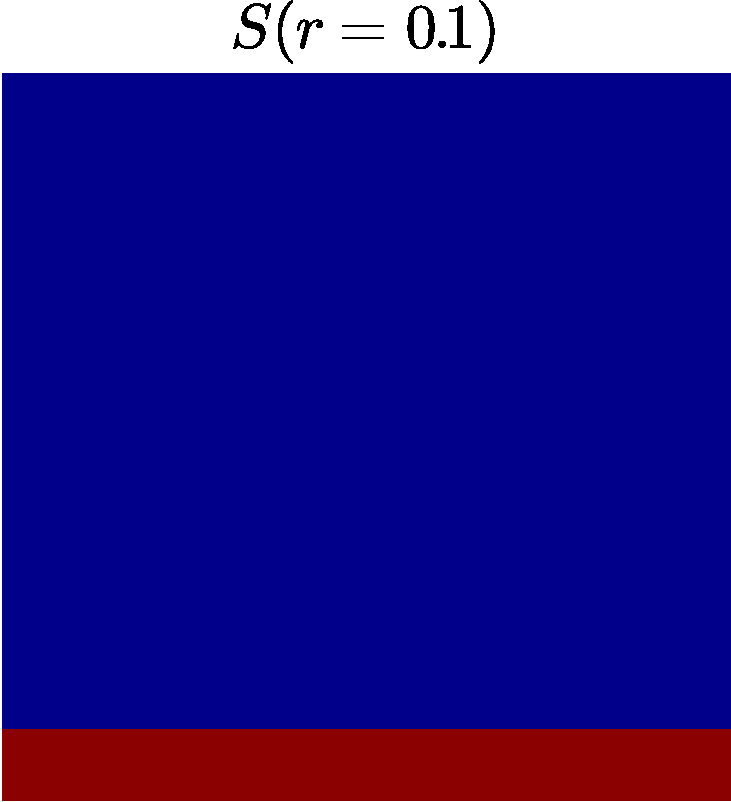
\includegraphics[width=0.4\columnwidth]{figs/strategy_entropy_S_r01.pdf}
	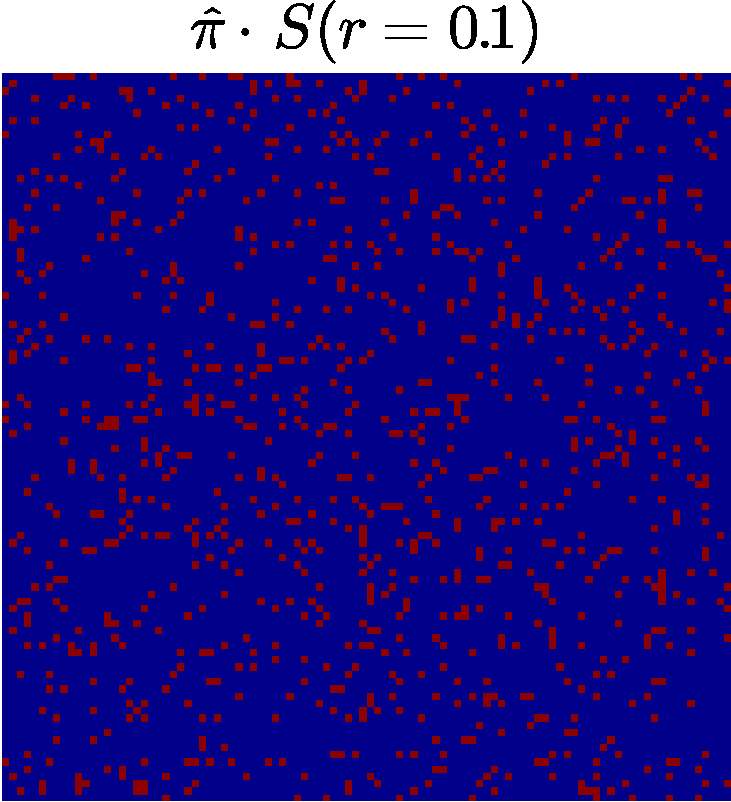
\includegraphics[width=0.4\columnwidth]{figs/strategy_entropy_R_r01.pdf}\\
	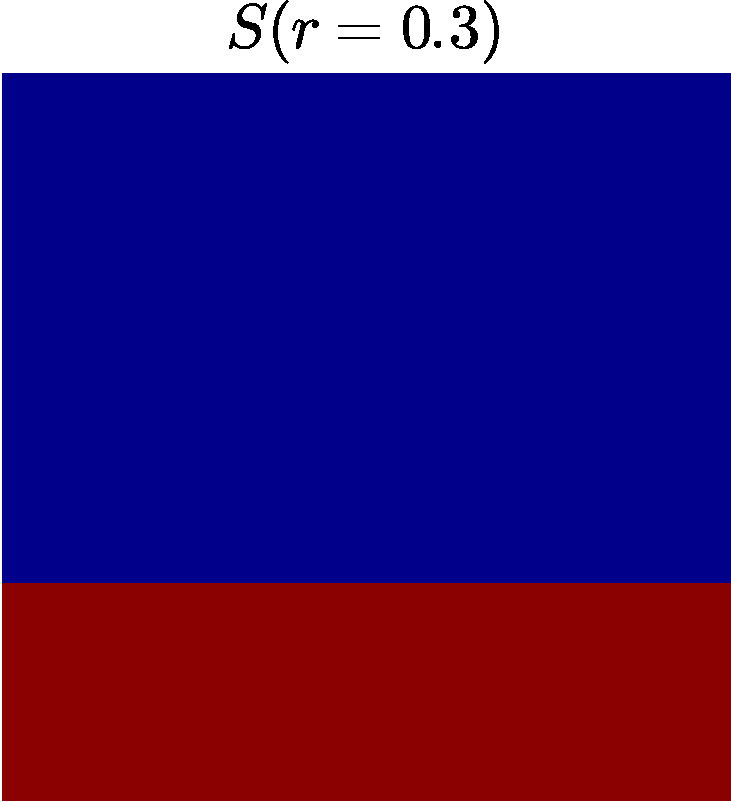
\includegraphics[width=0.4\columnwidth]{figs/strategy_entropy_S_r03.pdf}
	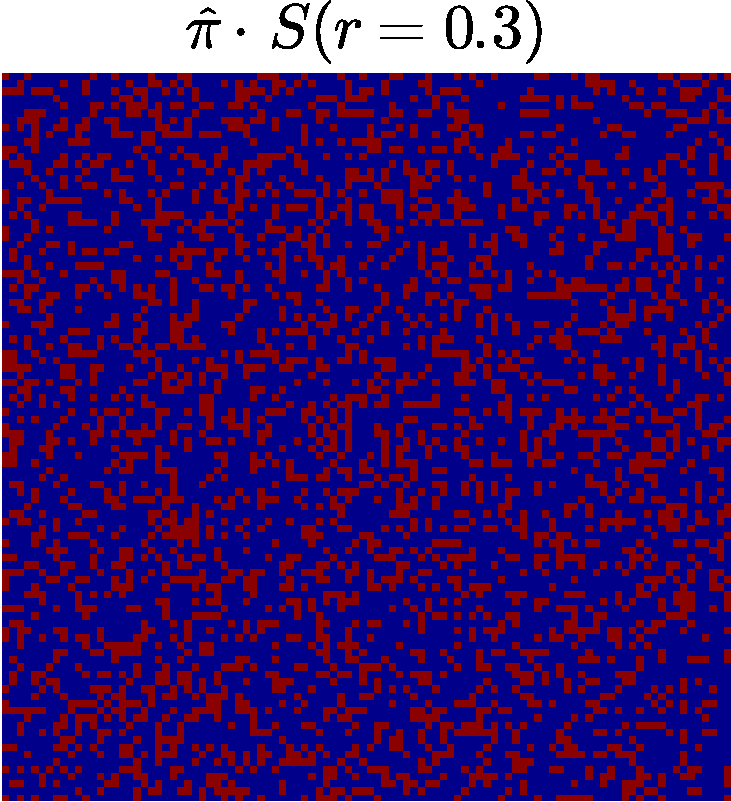
\includegraphics[width=0.4\columnwidth]{figs/strategy_entropy_R_r03.pdf}
	\caption{\textbf{Random sampling as a defence against strategic alignment.} (left) A minority of strategically aligned nodes may form false-majority if their alignment overlaps with a known allocation for consensus sets. (right) Random sampling erases strategic alignment and ensures node honesty is sampled with average-case $r$.} \label{fig:strategy_entropy}
\end{figure}

To uphold the integrity of majority votes, we require the likelihood of a minority gaining false-majority by chance to be upper-bounded by an exponentially small threshold $\varepsilon = 2^{-\lambda}$,
\begin{align}
	P_C(N,r) & \leq\varepsilon,
\end{align}
for statistical security parameter $\lambda>1$, a subjective parameter which may be application- or user-dependent. %As more stringent $\varepsilon$ implies larger $N_C$ hence workload, the cost of consensus is parameterised by $\varepsilon$.

We define the required consensus set size, $N_C$, as the smallest set size satisfying this inequality,
\begin{align}
	N_C(r,\varepsilon) & = \underset{N\in\mathbb{Z}^+}{\arg\min}(P_C(N,r)\leq\varepsilon).
\end{align}

For consensus to maintain $\varepsilon$-security, consensus sets should never be smaller than $N_C$. Simultaneously, choosing consensus sets larger than $N_C$ is unnecessary and wasteful. Tradeoff curves for $N_C(r,\varepsilon)$ are shown in Fig.~\ref{fig:P_M}.

This relationship can be conceptualised in terms of the mean and variance of $r$. The population (i.e whole-network) mean of $r$ is given by,
\begin{align}
	\mu_{\mathrm{pop}}(r) &= \frac{N_D}{N},
\end{align}
where there are $N_D$ dishonest nodes within a network of $N$ nodes. While \mbox{$N_D<N/2$} guarantees \mbox{$\mu_\mathrm{pop}(r)<1/2$}, thereby upholding majority rule on average, the sample variance, \mbox{$\sigma_{\mathrm{samp}}^2(r)$}, characterises deviation from the mean, affording the statistical opportunity for false-consensus,
\begin{align}
	\sigma_{\mathrm{samp}}^2(r) &= \frac{\sigma_{\mathrm{pop}}^2}{N_C},
\end{align}
where \mbox{$\sigma_{\mathrm{pop}}^2(r)$} is the population variance and $N_C$ is consensus set size, equivalently the number of random samples. Since \mbox{$\sigma_{\mathrm{samp}}^2(r)=O(1/N_C)$} scales inversely with consensus set size, larger consensus sets increase statistical confidence that the sample mean is close to the population mean, \mbox{$\mu_\mathrm{samp}(r)\approx \mu_\mathrm{pop}(r)$}.

Specifically, the probability that the sample mean positively deviates from the population mean by at least $d$ is,
\begin{align}
	\mathbb{P}(\mu_\mathrm{samp}(r)-\mu_\mathrm{pop}(r)\geq d) = \Phi\left(-\frac{d\sqrt{N_C}}{\sigma_\mathrm{pop}}\right)	,
\end{align}
where $\Phi(z)$ is the cumulative distribution function of the standard normal distribution,
\begin{align}
	\Phi(z) &= \frac{1}{\sqrt{2\pi}} \int_{-\infty}^z e^{-t^2/2}\,dt \nonumber\\
	&= \frac{1}{2} + \frac{1}{2} \mathrm{erf}\left(\frac{z}{\sqrt{2}}\right).
\end{align}
False-consensus requires \mbox{$\mu_\mathrm{samp}(r)>1/2$}, equivalently \mbox{$d=1/2-\mu_\mathrm{pop}(r)$}. Hence,
\begin{align}
	\mathbb{P}(\mu_\mathrm{samp}(r)\geq 1/2) = \Phi\left(\frac{\left(\mu_\mathrm{pop}(r)-\frac{1}{2}\right)\sqrt{N_C}}{\sigma_\mathrm{pop}}\right).
\end{align}
For whole-network consensus where \mbox{$N_C=N$} the sample and population means converge, \mbox{$\mu_\mathrm{samp}(r)=\mu_\mathrm{pop}(r)$}.

%\footnote{The number of distinct partitions of a set of nodes $\mathcal{S}$ into consensus sets of sizes $\{|\mathcal{C}_i|\}$ where,
%\begin{align}
%		|\mathcal{S}| = \sum_i |\mathcal{C}_i|,
%\end{align}
%is given by,
%\begin{align}
%	\# = \prod_i \binom{|\mathcal{S}|-\sum_{j=1}^{i-1}|\mathcal{C}_j|}{|\mathcal{C}_i|}.
%\end{align}
%}

\begin{figure}
	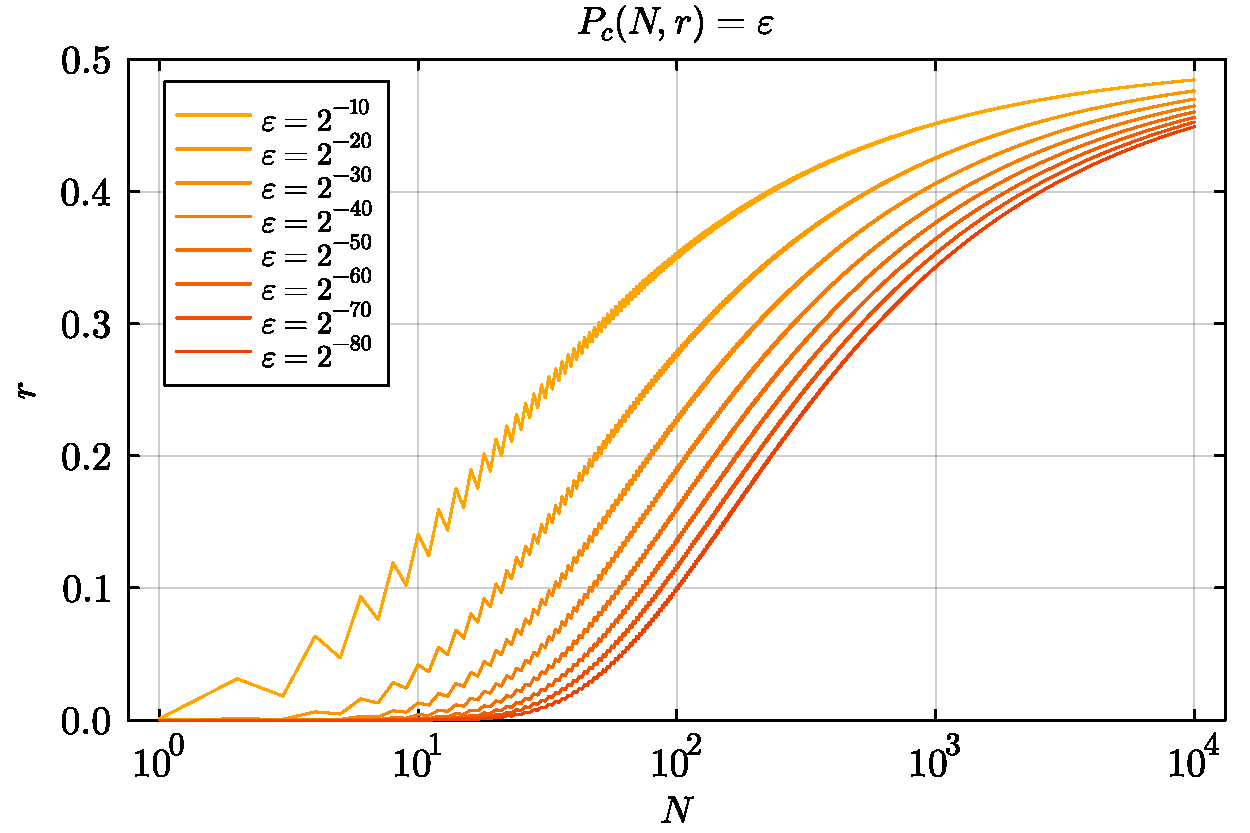
\includegraphics[width=\columnwidth]{figs/majority_prob.pdf}\\
	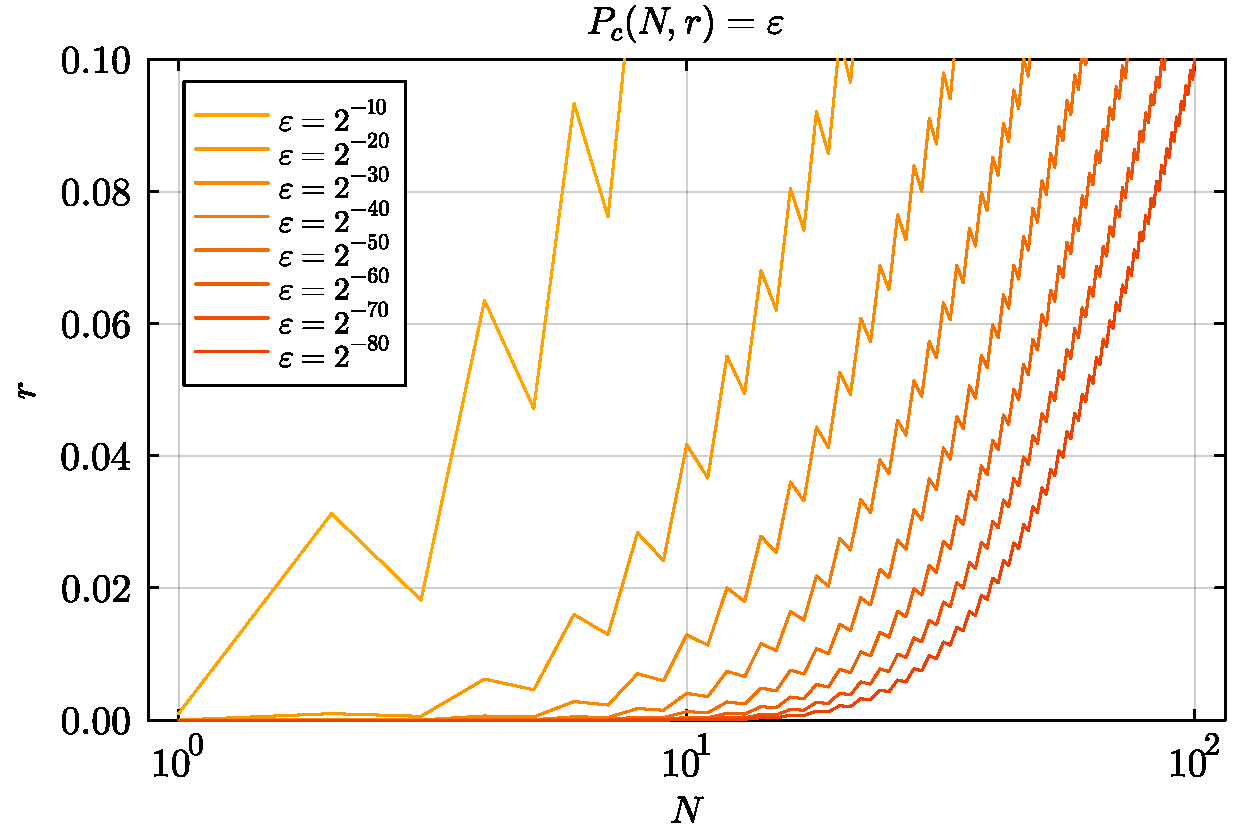
\includegraphics[width=\columnwidth]{figs/majority_prob_zoom.pdf}
	\caption{\textbf{Security tradeoffs with consensus set size.} $P_C(N,r)\leq\varepsilon$ is the probability that dishonest nodes within a random subset of size $N$ form a false-majority when the proportion of dishonest nodes is $r$, where $\varepsilon=2^{-\lambda}$ is the statistical security parameter. The oscillatory artefacts are associated with the non-linearity of \mbox{$\lfloor N/2\rfloor$} for even- and odd-valued $N$.} \label{fig:P_M}
\end{figure}

* Discussion on network diversity. Unenforceable in open, anonymous networks. $\mu(r)$ is not inherently a function of the number of nodes, but their diversity of control. In the Bitcoin network the injection of new nodes in the form of large mining pools can be antithetical to this. Common ownership implies correlated $r_i$ in an adversarial model.

\subsection{Centralised algorithm}

The random subset problem has a trivial centralised solution (Alg.~\ref{alg:random_subset}). We assign unique random bit-strings to each node, order them by their random number, and partition the ordered list piecewise into units of length $N_C$. These partitions form non-intersecting random subsets, each defining an independent consensus set.

\begin{algorithm}[H]
	\begin{algorithmic}
		\Function{RandomSubsets}{$\mathcal{S}$, $\{|\mathcal{C}|\}$} $\to \{\mathcal{C}\}$
		\LComment{Assign a random number to each node}
		\For{$i\in\mathcal{S}$}
		\State $\mathtt{random}_i \gets \textsc{Random}(\{0,1\}^n)$	\EndFor
		\LComment{Sort nodes by their random number}
		\State{$\mathtt{ordered}$ = \textsc{Sort}($\mathcal{S}$, $\mathtt{random}$)}
		\LComment{Partition the list into consensus sets}
		\State{$\{\mathcal{C}\}$ = \textsc{Partition}(\texttt{ordered}, $\{|\mathcal{C}|\}$)}
		\State \Return{$\{\mathcal{C}\}$}
		\EndFunction
	\end{algorithmic}
	\caption{Centralised algorithm for the random subset problem, assigning a set of nodes $\mathcal{S}$ to a set of independent random subsets $\{\mathcal{C}\}$ of given sizes $\{|\mathcal{C}|\}$.} \label{alg:random_subset}
\end{algorithm}

The challenge is to securely implement this algorithm in a decentralised environment, such that nodes are unable to compromise the randomness of the assignments of consensus sets.

\subsection{Proof-of-work} \label{sec:PoW}

* Hashcash: \cite{powemail, hashcash}

Proof-of-work has been widely employed in blockchains such as Bitcoin \cite{Nakamoto08} as a distributed protocol for choosing random subsets of nodes. Here, nodes compete to find satisfying inputs to hash functions whose outputs satisfy a constraint dictating the likelihood of success. This distributed algorithm effectively asks nodes to find solutions to randomised problems with very low probability of success, $p_\mathrm{mine}\ll 1$, such that winners are randomly allocated across nodes in the network.

Since hash functions are pseudo-random and exhibit pre-image resistance\footnote{For $\textsc{Hash}(x)\to y$ it is computationally hard to find a satisfying input $x\in\{0,1\}^*$ for given output $y\in\{0,1\}^n$.}, the only viable approach to finding such solutions is via brute-force, repeatedly hashing random bit-strings until a satisfying input is found. Winning nodes are hence allocated at random and cannot be spoofed under a computational hardness assumption. The distributed algorithm for proof-of-work is shown in Alg.~\ref{alg:PoW}.

\begin{algorithm}[H]
	\begin{algorithmic}
		\Function{ProofOfWork}{$\mathcal{S}$, \texttt{id}, \texttt{size}} $\to \mathcal{C}$
		\State $\mathcal{C} = \{\}$ \Comment{Consensus set}
		\While{$|\mathcal{C}|<\mathtt{size}$}
		\For{$i\in\mathcal{N}$} \Comment{In parallel}
		\State $\mathtt{random}_i = \textsc{Random}(\{0,1\}^n)$
		\State $\mathtt{output}_i = \textsc{Hash}(\mathtt{id}\,||\,\mathtt{random}_i)$
		\If{$\textsc{Valid}(\mathtt{output}_i)$}
		\State $\mathcal{C} \gets \mathcal{C} \cup \mathcal{S}_i$
		\EndIf
		\EndFor
		\EndWhile
		\State \Return{$\mathcal{C}$}
		\EndFunction
		\State
		\Function{Valid}{$x\in\{0,1\}^n$} $\to \{0,1\}$
		\If{$x/2^n \leq p_\mathrm{mine}$}
		\State \Return{\texttt{true}}
		\Else
		\State \Return{\texttt{false}}
		\EndIf
		\EndFunction
	\end{algorithmic}
	\caption{Random subsets via proof-of-work. Nodes $\mathcal{S}$ hash random bit-strings, salted by a problem instance specified by the previous block $\mathtt{id}$, where the per-hash success rate is $p_\mathrm{mine}$.} \label{alg:PoW}
\end{algorithm}

Proof-of-work has no requirement that nodes be known or trusted, providing a very general protocol suited to open networks in which anyone can participate. However, while affording a distributed solution to the random subset problem, this approach is inherently wasteful. The expected mining rate is,
\begin{align}
	R_\mathrm{mine} = p_\mathrm{mine}\cdot R_\mathrm{hash},
\end{align}
where $R_\mathrm{hash}$ is the network's net hash-rate\footnote{Bitcoin's cumulative network hash-rate was $\sim$500EH/s \mbox{($500\times 10^{18}\mathrm{H/s}$)} as of January, 2024 \cite{hashrate}.}. To inhibit the formation of multiple, simultaneous consensus sets (double-mining), potentially manifesting itself as forks in the blockchain, proof-of-work systems may introduce \emph{friction} by algorithmically adjusting the \emph{difficulty parameter} to ensure consistent mining times. To achieve constant mining time, difficulty must scale with cumulative network hash-rate, making the distributed algorithm less efficient as network size grows. For example, maintaining constant mining rate implies efficiency scales inversely with network size,
\begin{align}
	p_\mathrm{waste}=1-O\left(\frac{1}{n}\right),
\end{align}
asymptotically perfectly inefficient.

\subsection{Secure shared randomness} \label{sec:secure_shared_randomness}

An environment comprising a network of known nodes affords a more efficient solution to the random subset problem. The key observation is to utilise  \emph{secure shared randomness} to randomly permute and partition sets of nodes as per Alg.~\ref{alg:random_subset}. The source of shared randomness should be secure, in the sense that its randomness be robust against manipulation by dishonest nodes.

Secure shared randomness can be achieved by first requiring network nodes ($\mathcal{N}$) to present transaction \texttt{id}s whose hashes act as unique random numbers,
\begin{align}
	\mathcal{X}_i &= \textsc{Hash}(\mathtt{id}_i).\end{align}
A global key is then defined relative to the set $\mathcal{N}$ as,
\begin{align} \label{eq:global_K}
	\mathcal{X}_\mathcal{N} = \textsc{Hash}\left[\underset{i\in\mathcal{N}}{\big{|}\big{|}} \mathcal{X}^{\downarrow}_i\right],
\end{align}
our shared random source, where ${||}_i$ denotes concatenation over elements $i$, and \mbox{$\chi^{\downarrow}=\textsc{Sort}(\chi)$} denotes the sorted set.

\textbf{FIX ???}
Under the rules of entropy addition (Sec.~\ref{sec:entropy_add}), the randomness of the global key, $\mathcal{X}_\mathcal{N}$, cannot be compromised unless all $\mathcal{X}_i$ are compromised.

\subsection{Secure random subsets} \label{sec:hash_based_random_subsets}

* Change 'global key' to 'secure shared random source'.

From a secure global key, $\mathcal{X}_\mathcal{N}$, as per Eq.~\eqref{eq:global_K} the random subset problem affords a simple solution. Individual keys are assigned to each node,
\begin{align}
	K_i = \textsc{Hash}(\mathcal{X}_\mathcal{N} || \mathcal{X}_i).
\end{align}
Ordering and partitioning nodes by their associated $\{K_i\}$ assigns them to consensus sets as per Alg.~\ref{alg:random_subset}.

Multiple random subset allocations may be derived from a single global key by rehashing individual keys,
\begin{align}
	K_i^{(n)} = \textsc{Hash}^n(\mathcal{X}_\mathcal{N} || \mathcal{X}_i),
\end{align}
where $K_i^{(n)}$ denote keys for the $n$th round.

While nodes may choose their contributed \texttt{id}s, thereby influencing the established random source, $\mathcal{X}_\mathcal{N}$, this does not provide an avenue for compromising the integrity of random subset assignment. Adversarial nodes attempting to compromise $\varepsilon$-security by manipulating $\mathcal{X}_\mathcal{N}$ must find the necessary satisfying pre-images $\mathtt{id}_i$. Searching over $\mathrm{poly}(\lambda)$ pre-images, each associated with unique, independently random instances of $\mathcal{X}_\mathcal{N}$, preserves the exponentially decreasing likelihood of compromise,
\begin{align}
	\varepsilon' \leq \frac{\mathrm{poly}(\lambda)}{2^\lambda}.
\end{align}

This approach to random subset assignment necessarily assumes a collectively agreed upon known set of nodes, as the global key $\mathcal{X}_\mathcal{N}$ cannot be established from an undefined set, nor can an undefined set be ordered.

%\subsection{Quantum-random subsets} \label{sec:QRSS}
%
%Hash-based random subsets inherit their security from the pre-image resistance and pseudo-random characteristics of hash functions. While these assumptions are strongly believed to be sound, they nonetheless afford only computational security.
%
%Ideal implementation of the random subset problem demands information-theoretic security, achievable with the introduction quantum random number (QRN) sources. 
%

%Quantum random numbers exhibit in-principle maximum entropy, affording classical networks the ability to observe 

%Since uniformly distributed QRNs exhibit maximum entropy, a global key $X_\mathcal{S}$ established via Eq.~\eqref{eq:global_K} will be quantum-random if at least one $X_i$ was.

%\subsubsection{Quantum-random permutations}
%
%Established max-entropy global key must be mapped to node-permutations. Consider the space of bit-strings of length $n$,
%\begin{align}
%	X = \{0,1\}^n,\,\, |X| = 2^n,
%\end{align}
%and the space of permutations over $m$ elements, given by the symmetric group of degree $m$,
%\begin{align}
%	\pi \in S_m,\,\, |S_m| = m!.
%\end{align}
%Uniquely mapping bit-strings to permutations, $K \mapsto S_m$, requires the order of their domains scale in tandem following a pigeonhole argument,
%\begin{align}
%	|X| = |S_m|.
%\end{align}
%The required number of QRN bits therefore scales as,
%\begin{align}
%	n = \log_2(m!),
%\end{align}
%from which random node-permutations may be assigned via,
%\begin{align}
%	K_i = X_{\pi_i}.
%\end{align}
%The number of QRN bits required to implement a global node permutation is shown in Fig.~\ref{fig:bits_permutations}.
%
%\begin{figure}[!htb]
%	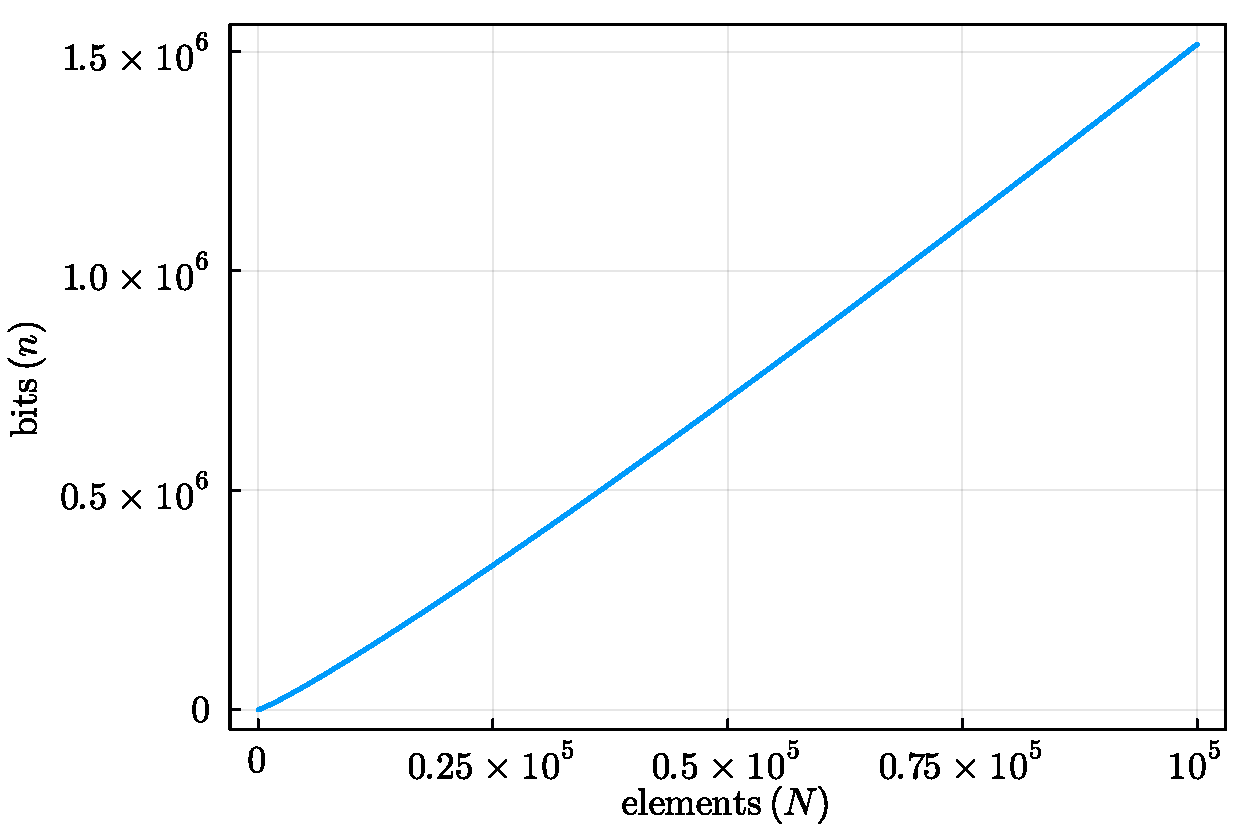
\includegraphics[width=\columnwidth]{figs/bits_permutations.pdf}
%	\caption{\textbf{Number of bits required to encode an arbitrary node permutation.} This upper-bounds the required $n$ for the consensus group.} \label{fig:bits_permutations}	
%\end{figure}

